\documentclass{article}
\usepackage{graphicx}
\usepackage[margin = 2cm]{geometry}
\usepackage{caption}
\usepackage{subcaption}

\title{PCO Laboratoire 5 \\
\large Modélisation par moniteur de Mesa}
\author{Benoît Delay, Eva Ray}

\begin{document}
\maketitle

\section*{Description des fonctionnalités du logiciel}

Le programme modélise une boutique de barbier. La boutique est constituée d'un salon dans lequel on trouve une salle d'attente avec
un nombre de siège fixes et une chaise de travail sur laquelle un client peut se faire couper les cheveux. Un certain nombre de clients
vont tenter de se faire couper les cheveux par le barbier. Le programme est doté d'une interface graphique, qui est animée grâce aux
annimations présentes dans la clase \texttt{PcoSalon} qui représentent les actions du barbier et des clients. \\

Les fonctionnalités du salon sont assez représentatives d'un salon de coiffure classique. Le salon est géré par un barbier qui s'occupe
de couper les cheveux des clients sur la chaise de travail. Lorsqu'il a fini de s'occuper d'un client, le barbier appelle le prochain client
parmi ceux qui sont en train d'attendre dans la salle d'attente. Le barbier fait bien attention à appeler les clients dans leur ordre
d'arrivée. S'il n'y a plus aucun client dans la salle d'attente, le barbier va faire une petite sieste et ne revient que lorsqu'un nouveau
client arrive à la porte de la boutique. Le comportement du barbier est simulé par la méthode \texttt{Barber::run()}. \\

Les clients, quant à eux, ont aussi un comportement prédéfini. Les clients qui souhaitent se faire couper les cheveux ne peuvent entrer
dans le salon que si celui-ci a assez de place pour les acueillir, c'est-à-dire s'il y a de la place dans la salle d'attente ou si aucun
client n'est présent dans le salon. Dans le second cas, la barbier est en train de faire une petite sieste, comme mentionné ci-dessus.
L'arrivée du nouveau client à la porte va réveiller le barbier qui se déplace jusqu'à la chaise de travail, où le nouveau client
va le rejoindre. Si le salon est plein, le
client va faire un petit tour avant de revenir voir si une place s'est libérée. Si le client accède à la salle d'attente, il va gentiment
s'asseoir sur une chaise libre et attend que le barbier l'appelle. Lorsque c'est le tour du client, il se dirige vers la chaise de travail,
où le barbier lui coupe les cheveux. Une fois la coupe finie, le client quitte le salon et attend que ses cheveux repoussent avant de
revenir se faire faire une nouvelle coupe. Le comportement d'un client est simulé par la méthode \texttt{Client::run()} \\

Les comportements décrits ci-dessus sont représentés par les méthodes de la clase \texttt{PcoSalon} et correspondent aux machines d'états
illustrées ci-dessous. \\

La terminaison du programme est gérée grâce aux méthodes \texttt{PcoSalon::endService()} et \\ \texttt{PcoSalon::isInService()}.
La fin du programme
est innitiée dès qu'une entrée utilisateur est déclenchée dans le terminal. Le salon est alors fermé. Les clients qui ne se trouvent pas
actuellement dans le salon rentrent chez eux. Le barbier finit de s'occuper de tous les clients qui sont encore dans le salon mais n'en
accepte pas de nouveau. Une fois qu'il a terminé son travail, ferme le salon et termine sa journée. \\

Le logiciel simule le comportement du barbier et des clients par des threads différents, il est donc multi-threadé. Par conséquent, il doit 
assurer une bonne gestion de la concurrence pour les ressources partagées entre plusieurs threads. Les méthodes du salon sont ainsi implémentées 
à l'aide d'un moniteur de Mesa, qui permet de gérer la concurrence et les animations. 

\begin{figure}
    \centering
        \begin{subfigure}[b]{0.4\textwidth}
        \centering
        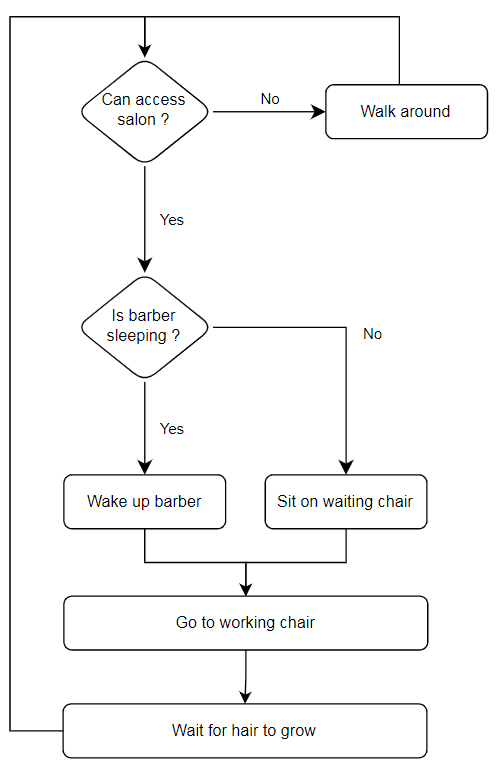
\includegraphics[width=\textwidth]{figures/machine_etat_client.png}
        \caption{Machine d'état du client}
        \label{fig:machine état client}
    \end{subfigure}
    \hfill
    \begin{subfigure}[b]{0.4\textwidth}
        \centering
        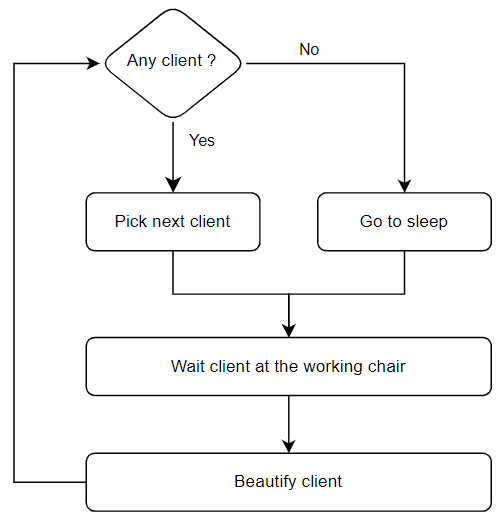
\includegraphics[width=\textwidth]{figures/machine_etat_barbier.png}
        \caption{Machine d'état du barbier}
        \label{fig:machine état barbier}
    \end{subfigure}
\end{figure}

\section*{Choix d'implémentation}
% Comment avez-vous abordé le problème, quels choix avez-vous fait, quelle 
% décomposition avez-vous choisie, quelles variables ont dû être protégées, ...

\subsection*{Variables de condition}

La synchronisation entre les différents threads du programme se fait via des variables de condition qui sont des attributs
protégés de la classe \texttt{PcoSalon}.

\begin{itemize}
    \item \texttt{canGoForHaircut}: La variable de condition \texttt{canGoForHaircut} représente l'attente d'un client sur une des chaises 
    de la salle d'attente avant de pouvoir aller se faire couper les cheveux. Les threads des clients attendent sur cette variable de 
    condition dans la méthode \texttt{PcoSalon::accessSalon} et le barbier réveille les threads des clients en attente depuis la méthode 
    \texttt{PcoSalon::pickNextClient}.
    \item \texttt{waitClient}: La variable de condition \texttt{wairClient} représente le fait que le barbier attente qu'un client se déplace
    de la salle d'attente à la chaise de travail. Le thread du barbier attent sur cette variable de condition dans la méthode \texttt{PcoSalon::waitClientAtChair} et le 
    client signifie qu'il a atteint la chaise de travail dans la méthode \texttt{PcoSalon::goForHaircut}.
    \item \texttt{doneBeautified}: La variable de condition \texttt{doneBeautified} représente le fait qu'un client attendre que sa coupe de
    cheveux se termine. Le thread du client attent sur cette variable de condition dans la méthode \texttt{PcoSalon::goForHaircut} et le 
    barbier signifie au client qu'il a finit la coupe dans la méthode \\ \texttt{PcoSalon::beautifyClient}. 
    \item \texttt{barberSleeping}: La variable de condition \texttt{barberSleeping} représente le sommeil du barbier. Le thread du barbier attent sur cette variable 
    de condition dans la méthode \texttt{PcoSalon::goToSleep} pour représenter la fait que le barbier s'endort. Le 
    client signifie que le barbier doit se réveiller dans la méthode \\ \texttt{PcoSalon::accessSalon}.
\end{itemize}

\subsection*{Gestion des chaises de la salle d'attente}
Pour gérer les chaises de la salle d'attente, nous avons ajouté un attribut \texttt{chairs} dans la classe \texttt{PcoSalon}. C'est
simplement un vecteur de booléens qui a pour taille le nombre de chaises de la salle d'attente. Si le booléen contenu à l'indice i
vaut \texttt{false} cela signifie que la chaise numéro i est libre, s'il vaut \texttt{true} cela signifie que la chaise est occupée.
Dans la méthode \texttt{PcoSalon::accessSalon}, on assigne une chaise libre au client qui doit aller s'asseoir dans la salle d'attente,
elle devient alors occupée. Lorsque le client se déplace sur la chaise de travail, on libère la chaise sur laquelle il était assis.   

\subsection*{Gestion de la file FIFO}

Une des fonctionnalités du programme est d'assurer le fait que le barbier s'occupe des clients dans leur ordre d'arrivée dans le salon. Pour ce faire,
nous avons implémenter une file FIFO avec une méthode de ticketing. L'idée est simple; chaque client qui arrive dans la salle d'attente prend un ticket à
la machine à tickets, représentée par l'attribut \texttt{ticketMachine} de la classe \texttt{PcoSalon}. Il attend ensuite sur la variable de condition 
\texttt{canGoForHaircut}. Lorsqu'il est prêt, le barbier va \texttt{notifyALL} sur cette variable, ce qui va avoir pour conséquence de réveiller tous les 
threads en attente. A ce moment, le client réveillé va comparer son numéro de ticket avec celui stocké dans l'attribut \texttt{nextClient} de la 
classe \texttt{PcoSalon} qui représente le numéro du prochain client à pouvoir aller se faire couper les cheveux. Si les numéros coïncident, le client
peut aller se faire couper les cheveux et l'attribut \texttt{nextClient} est incérmenté, sinon, il se remet en attente jusqu'à ce que ce soit son tour.  

\subsection*{Gestion de l'interruption du programme}

La terminaison du programme est amorcée lorsqu'une entrée utilisateur est déclenchée dans le terminal. Elle est gérée grâce aux méthodes 
\texttt{PcoSalon::endService()} et \texttt{PcoSalon::isInService()}. Nous avons ajouté un attribut booléen \texttt{isOpen} dans la classe \texttt{PcoSalon} 
qui vaut \texttt{true} lorsque le salon est ouvert et \texttt{false} sinon. La méthode \texttt{PcoSalon::isInService()} renvoie simplement cet attirbut. Elle nous
permet de connaître l'état d'ouverture du salon depuis l'extérieur de la classe. Dans la méthode \texttt{PcoSalon::endService()} on change la valeur de 
\texttt{isOpen} à \texttt{false} pour informer de la fermeture du salon. On s'assure aussi de gérer le cas dans lequel la fermeture du salon est 
déclenchée lorsque le barbier est en train de dormir. Dans ce cas, on réveille le barbier pour que son thread puisse se finir et ne pas rester en 
attente indéfiniment sur la variable de condition \texttt{barberSleeping}. 
On s'assure ensuite dans la méthode \texttt{Barber::run} du barbier qu'il s'occupe des clients qui sont étaient déjà présents dans la salon avant la
fermeture avant que son thread ne s'arrête pour de bon. Cela est mis en place grâce aux méthodes \texttt{PcoSalon::isInService()} et
\texttt{PcoSalon::getNbClient()}. Les clients attendent encore que leur cheveux repoussent avant de se rendre compte que le salon est fermé et rentrer 
chez eux pour de bon.

\subsection*{Autres choix}

\begin{itemize}
    \item Nous sommes partis du principe que le client qui réveille le barbier ne va pas s'asseoir dans la salle d'attente mais attend
    à la porte que le barbier ait atteint la chaise de travail avant de l'y rejoindre.
    \item Nous avons traité le cas où il n'y a aucune chaise dans la salle d'attente. Dans ce cas, le client qui arrive à la porte 
    réveille le barbier, attend à la porte que le barbier ait atteint la chaise de travail avant de l'y rejoindre. Le barbier va aller
    dormir entre chaque client, puisqu'il n'y a techniquement aucun client dans le salon dans cette situation. L'attribut booléen 
    \texttt{clientWaitingAtDoor} de la classe \texttt{PcoSalon} nous permet de gérer ce cas particulier en le mettant à jour correctement. 
\end{itemize}

\section*{Tests effectués}
% Description de chaque test, et information sur le fait qu'il ait passé ou non

Le résultat des tests ci-dessus a notamment pu être vérifié car nous logons dans l'interface graphique des informations sur la plupart des 
actions entreprises par le barbier et les clients. En particulier, en plus de décrire leur comportement, un message s'affiche lorsque
les threads des clients ou du barbier se finissent.

\subsection*{Test: Fonctionnalités du salon}

\subsubsection*{Paramètres par défaut}

Les tests suivants ont été effectués avec les paramètres par défaut, c'est-à-dire avec 10 clients et 2 sièges dans la salle d'attente

\begin{itemize}
    \item Lorsqu'un client souhaite accéder au salon et que le barbier est en train de dormir, le barbier se réveille et se déplace
    vers la chaise de travail. Le client attend sur le pas de la porte que le barbier soit arrivé à la chaise et l'y rejoint lorsque
    c'est le cas. C'est le comportement attendu.
    \item Lorsqu'un client souhaite accéder au salon alors que le barbier est déjà réveillé et qu'il y a de la place dans la 
    salle d'attente, le client va s'asseoir sur une chaise libre de la salle d'attente et attend son tour. 
    C'est le comportement attendu.
    \item Lorsqu'un client souhaite accéder au salon alors que le barbier est déjà réveillé et qu'il n'y a pas de place dans la 
    salle d'attente, le client ne peut pas accéder au salon et va faire un tour avant de rententer sa chance. 
    C'est le comportement attendu.
    \item Lorsqu'il n'y a plus aucun client dans le salon, le barbier va faire une sieste. C'est le comportement attendu.
    \item Lorsqu'on lance le programme, le barbier commence toujours par aller faire une sieste. C'est le comportement attendu.
    \item Lorsque le barbier appelle le prochain client, il attend que le client arrive sur la chaise de travail avant de commencer la coupe.
    C'est le comportement attendu.
    \item Lorsque le barbier appelle le prochain client, c'est le client qui est arrivé le premier dans le salon qui se dirige vers la chaise
    de travail. C'est le comportement attendu.
    \item Lorsque le barbier est en train de faire une coupe, aucun autre client ne peut se diriger vers la chaise de travail tant 
    qu'il n'a pas fini. C'est le comportement attendu.
    \item Lorsque le client a une nouvelle coupe, il quitte le salon et attend que ses cheveux repoussent avant d'essayer d'accéder 
    à nouveau au salon.
\end{itemize}

\subsubsection*{Variation des paramètres}

Les tests suivants ont été réalisés en modifiant les paramètres par défaut pour tester la robustesse du programme.

\begin{itemize}
    \item Lorsqu'il n'y a aucun siège dans la salle d'attente, le client va toujours devoir réveiller le barbier et attendre à la porte.
    Lorsque le barbier a fini la coupe du client, il repart tout de suite dormir avant de se faire rapidement réveiller par le prochain
    client qui attend à la porte. C'est le comportement attendu. 
    \item Lorsqu'il n'y a qu'un seul client et 2 (ou un autre nombre non nul) de sièges dans la salle d'attente, le client réveille
    le barbier et attend à la porte. Le client ne va pas attendre dans la salle d'attente mais reste à la porte. Entre chaque coupe de 
    l'unique client, le barbier va dormir. C'est le comportement attendu.
    \item Lorsqu'il y a 2 client et 2 sièges dans la salle d'attente (c'est-à-dire autant de clienst que de chaises), le programme se 
    déroule conformément au cahier des charges. C'est le comportement attendu.
    \item Lorsqu'il n'y a aucun client, le babrier va dormir et ne se réveille jamais. C'est le comportement attendu. 
    \item Lorsqu'il y a plus de 2 chaises dans la salle d'attente et 10 clients, les clients s'asseyent toujours sur une chaise libre et 
    sont toujours appelés par le barbier dans leur ordre d'arrivée. C'est le comportement attendu.
    \item Lorsqu'un met 20 clients et 2 chaises dans la salle d'attente, le programme se déroule conformément au cahier des charges.
    C'est le comportement attendu.
\end{itemize}

\subsection*{Test: Terminaison du programme}

La fin des threads peut être vérifiée car un message est logé dans l'interface graphique dans les cases réservées aux clients et au barbier. 
Un message signifiant la terminaison du programme (qui était déjà présent lorsque nous avons reçu le squelette du labo) apparait aussi 
dans le terminal.

\begin{itemize}
    \item Lorsque le barbier est en train de travailler et une entrée utilisateur est déclenchée dans la console, plus aucun nouveau client
    ne rentre dans le salon, le barbier finit de s'occuper du client qui est actuellement sur la chaise de travail et de ceux qui sont
    en train d'attendre dans la salle d'attente avant que son thread se finissent. Le thread des clients qui n'étaient pas dans le salon au 
    moment de la terminaison du programme se finit dès que les clients constatent que le salon est fermé. Les clients qui étaient dans le
    salon au moment de la fermeture quittent le salon lorsque leur coupe est terminée et attendent encore une fois que leur cheveux repoussent
    avant que leur thread s'arrête lorsqu'ils constatent que le salon est fermé. Le message "le programme est terminé" apparait dans la console.
    C'est le comportement attendu.
    \item Lorsque le barbier est en train de dormir et une entrée utilisateur est déclenchée dans la console, il se réveille pour que son
    thread puisse se terminer. Le message "le programme est terminé" apparait dans la console. C'est le comportement attendu.
    \item Lorsqu'une entrée utilisateur est déclenchée alors que le barbier est en train d'attendre que le client arrive à la chaise de travail
    le programme se termine comme attendu. 
\end{itemize}

\section*{Conclusion}

Nous avons implémenté un programme multi-threadé qui simule un salon de coiffure conformément au cahier des charges. Nous avons implémenté une
gestion de la synchronisation grâce à des variables de condition d'un moniteur de Mesa qui semblent faire leur travail convenablement. 
L'accès des clients au salon, l'attente dans la salle d'attente, la prise en charge des clients, la coupe, la repouss des cheveux et le 
sommeil du barbier sont gérés correctement.
L'innitation de la fin de programme par le déclenchement d'une entrée utilisateur dans le terminal fonctionne comme espéré et permet de 
mettre fin aux threads de la simulation correctement.

\end{document}